\documentclass{article}
\usepackage{tikz}
\usepackage{animate}
\usepackage{amsmath}
\usepackage{ifthen}
\usepackage{pgfmath}
\usetikzlibrary {matrix}
\usepackage{tikzlings}
\usepackage{tikzlings-penguins}
\usepackage{graphics,graphicx}

\newcommand{\token}{
  \begin{scope}[node distance=0pt]
   \node[ rectangle,fill=red] at (0,0) {};
   \node[ rectangle,fill=red!20] at (1,0) {};
   \node[ rectangle,fill=red!40] at (2,0) {};
   \node[ rectangle,fill=blue!20] at (3,0) {};
   \node[ rectangle,fill=blue!40] at (4,0) {};
   \node[ rectangle,fill=blue] at (5,0) {};
   \end{scope}
}
\begin{document}
\begin{figure}
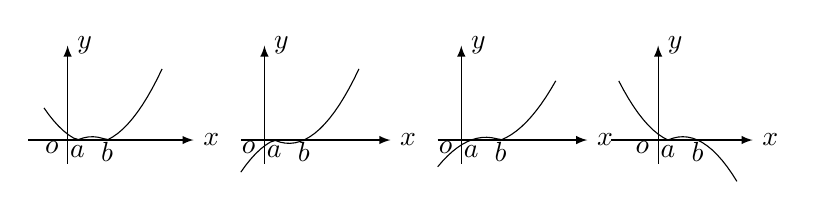
\begin{tikzpicture}[>=latex,domain=-0.3:1.2]
 \xdef\a{0.125} 
 \xdef\b{0.5}
 \xdef\scale{1.2}
 \xdef\ppos{-0.6}
  \begin{scope}
    \draw[->] (-0.5,0) -- (1.6,0) node[right] {$x$};
    \draw[->] (0,-0.3)--(0,1.2) node[right] {$y$};
    \node (a) at (\a,-0.15) {$a$};
    \node (b) at (\b,-0.15) {$b$};
    \node (o) at (-0.2,-0.1){ $o$};
    \draw plot (\x,{\scale*abs(\x-\a)*abs(\x-\b)});
  \end{scope}
  \begin{scope}[xshift=2.5cm]
    \draw[->] (-0.3,0) -- (1.6,0) node[right] {$x$};
    \draw[->] (0,-0.3)--(0,1.2) node[right] {$y$};
    \node (a) at (\a,-0.15) {$a$};
    \node (b) at (\b,-0.15) {$b$};
    \node (o) at (-0.2,-0.1){ $o$};
    \draw plot (\x,{\scale*abs(\x-\a)*(\x-\b)});
  \end{scope}
  \begin{scope}[xshift=5cm]
    \draw[->] (-0.3,0) -- (1.6,0) node[right] {$x$};
    \draw[->] (0,-0.3)--(0,1.2) node[right] {$y$};
    \node (a) at (\a,-0.15) {$a$};
    \node (b) at (\b,-0.15) {$b$};
    \node (o) at (-0.2,-0.1){ $o$};
    \draw plot (\x,{\scale(\x-\a)*abs(\x-\b)});
  \end{scope}
  \begin{scope}[xshift=7.5cm,domain=-0.5:1]
    \draw[->] (-0.6,0) -- (1.2,0) node[right] {$x$};
    \draw[->] (0,-0.3)--(0,1.2) node[right] {$y$};
    \node (a) at (\a,-0.15) {$a$};
    \node (b) at (\b,-0.15) {$b$};
    \node (o) at (-0.2,-0.1){ $o$};
    \draw plot (\x,{\scale*-1*abs(\x-\a)*(\x-\b)});
  \end{scope}
\end{tikzpicture}
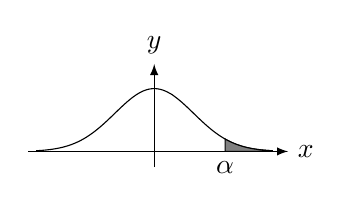
\begin{tikzpicture}[>=latex,domain=-3:3,x=0.5cm,y=2cm]
  \pgfmathparse{ {1.0/sqrt{2*pi}/4}}  
  \let\ymax\pgfmathresult
  \xdef\mr{1.8}
  \draw[->] (-3.2,0)--(3.4,0) node[right] {$x$};
  \draw[->] (0,-0.1) --(0,\ymax) node[above] {$y$};
  \draw[smooth,samples=100] plot (\x,{exp(-\x *\x/2)/sqrt(2*pi)});
  \filldraw[fill=gray,domain=\mr:3] (\mr,0) node[below] {$\alpha$} -- plot (\x,{exp(-\x *\x/2)/sqrt(2*pi)}) --(3,0)--cycle;
\end{tikzpicture}
\end{figure}
  \begin{center}
\begin{figure}
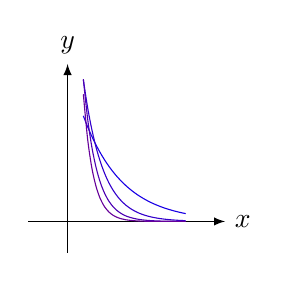
\begin{tikzpicture}[>=latex,x=0.5cm,y=2cm]
  \draw[->] (-1,0) --(4,0) node[right] {$x$};
  \draw[->] (0,-0.2) --(0,1) node[above] {$y$};
  \foreach \ll[evaluate=\ll as \c using 10*\ll] in {1,2,3,4}{
  \draw[domain=0.4:3,smooth,red!\c!blue] plot (\x, { \ll*exp(\ll*-\x)});
  }
\end{tikzpicture}
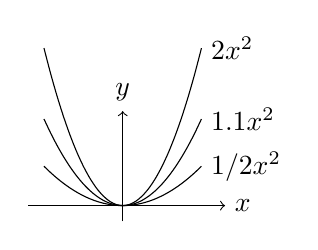
\begin{tikzpicture}
  \draw[->] (-1.2,0) --(1.3,0) node[right] {$x$};
  \draw[->] (0,-0.2) --(0,1.2) node[above] {$y$};
  \foreach \a in {1/2,1.1,2}{
   \draw[domain=-1:1,smooth] plot(\x, {\a*\x*\x}) node[right] {$\a x^2$};
  }
\end{tikzpicture}
\end{figure}
\end{center}

\begin{animateinline}[poster=first,autoplay, palindrome]{4}
\multiframe{3}{iangle=5+5}{
\begin{tikzpicture}[>=latex,x=0.5cm,y=2cm]
  \draw[->] (-1,0) --(4,0) node[right] {$x$};
  \draw[->] (0,-0.2) --(0,1) node[above] {$y$};
  \pgfmathparse{\iangle/5} 
  \let\ll\pgfmathresult
  \draw[domain=0.4:3,smooth,red!\iangle!blue] plot (\x, { \ll*exp(\ll*-\x)}) node[above right]{$\ll e^{-\ll x}$} ;
\end{tikzpicture}
}
\end{animateinline}
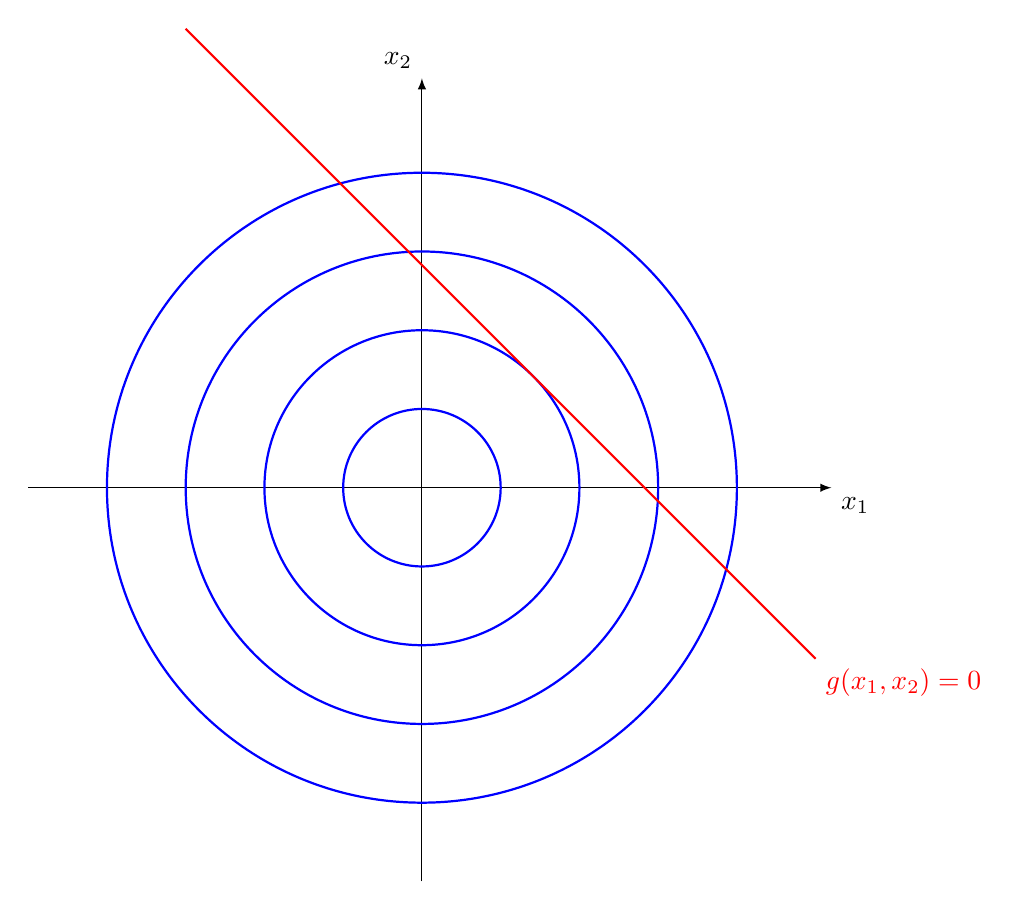
\begin{tikzpicture}[>=latex]
  \draw [->] (-5,0) --(5.2,0) node[below right]{$x_1$};
  \draw[->] (0,-5) --(0,5.2) node[above left] {$x_2$};
  \foreach \r in {1,2,3,4}{
   \draw[blue,thick]  (0,0) circle[radius=\r] ;
  }
  \pgfmathparse{sqrt(2)*2} 
  \let\ss\pgfmathresult 
  \draw [domain=-3:5,smooth,thick,red] plot(\x,{-\x + \ss}) node[below right] {$g(x_1,x_2)=0$};
\end{tikzpicture}

\begin{tikzpicture}
  \token ;
\end{tikzpicture}
\end{document}
